\documentclass{article}

% Language setting
% Replace `english' with e.g. `spanish' to change the document language
\usepackage[english]{babel}
\usepackage{hyperref}

% Set page size and margins
% Replace `letterpaper' with `a4paper' for UK/EU standard size
\usepackage[letterpaper,top=2cm,bottom=2cm,left=3cm,right=3cm,marginparwidth=1.75cm]{geometry}

% Useful packages
\usepackage{amsmath}
\usepackage{graphicx}
\usepackage[colorlinks=true, allcolors=blue]{hyperref}

\title{Verification of ACAS Xu using Alpha-Beta-Crown and Nnenum }
\author{Văduva Vlad-Andrei, Granu Dragoș Vlad, Iordache Constantin, Hrițu Toma\\[1cm]{\small Coordinator: Conf. dr. Erașcu Mădălina}}


\begin{document}
\maketitle
\newpage
\tableofcontents
\clearpage
\section{Abstract}
The purpose of verifying the ACAS Xu benchmark is to assure the correctness of the results output by the benchmark. Such results can have real life consequences. Therefore, it is important to ensure the validity of these results in order to further improve and develop the benchmark.

\section{Introduction}
ACAS Xu\cite{vnn} is an air-to-air collision avoidance system designed for unmanned aircraft that issues horizontal turn advisories to avoid an intruder aircraft. Due the use of a large lookup table in the design, a neural network compression of the policy was proposed. The purpose of this paper is to document the process of verifying the ACAS Xu benchmark using two VNN tools, alpha-beta crown and nnenum.

\section{ACAS Xu}
ACAS XU\cite{acasxu} refers to the Airborne Collision Avoidance System For Unmanned Aircraft. ACAS XU is a set of experimental enhancements to the existing ACAS II (Airborne Collision Avoidance System II ) used in aviation. ACAS is a safety system designed to reduce the risk of mid-air collisions between aircraft.

ACAS II is based on the Traffic Advisory (TA) and Resolution Advisory (RA) concepts. When ACAS II detects a potential collision threat, it provides pilots with advisories to take evasive action, such as a vertical resolution advisory to climb or descend.

ACAS XU represents advancements and upgrades to the existing system, incorporating improved algorithms and technologies to enhance collision avoidance capabilities. 

\subsection{Architecture Elements}
ACAS Xu uses FC and Relu for its architecture.\newline
FC is a Fully Connected layer inside the neural network. This is one one the layer types that is used as a basis in almost all neural networks. In an FC layer, all the neurons of the input are connected to every neuron of the output layer. In an FC layer, a weighted linear transformation is applied to the input neurons and then pass the output through a non-linear activation function.
\newline
ReLU\cite{relu} (Rectified Linear Unit) is an activation function that introduces the property of non-linearity to a deep learning model and solves the vanishing gradients issue.
\newpage
\section{Tools}
\subsection{Alpha-Beta-Crown}
Alpha-Beta-CROWN\cite{alpha-beta} is a neural network verification tool based on an efficient linear bound propagation framework and branch and bound. It can be accelerated efficiently on GPUs and scales well for big convolutional neural networks.\newline
Supported neural network architectures:
\begin{itemize}
\item Layers: fully connected, convolutional, pooling, transposed convolution
\item Activation functions: ReLU, sigmoid, tanh, arctan, sin, cos, tan
\item Residual connections and other irregular graphs
\end{itemize}
\newline
Prerequisites: Conda, miniconda works as well.\newline
Miniconda Installation:
We create a folder named miniconda3:

\begin{verbatim}mkdir -p ~/miniconda3\end{verbatim}
We must download miniconda from the main site:
\begin{verbatim}wget https://repo.anaconda.com/miniconda/Miniconda3-latest-Linux-x86_64.sh -O ~/miniconda3/miniconda.sh\end{verbatim}
We run the installation script:
\begin{verbatim}bash ~/miniconda3/miniconda.sh -b -u -p ~/miniconda3
\end{verbatim}

After we installed the prerequisites, we can proceed with alpha-beta-crown installation:
We clone the GitHub repository:
\begin{verbatim}git clone --recursive https://github.com/Verified-Intelligence/alpha-beta-CROWN.git\end{verbatim}
This way, we also clone auto-LiRPA sub-module, which will then be installed with the command \begin{verbatim} python setup.py install\end{verbatim}
Remove the old environment, if necessary:
\begin{verbatim}conda deactivate\end{verbatim}
\begin{verbatim}conda env remove --name alpha-beta-crown\end{verbatim}

Install all dependents into the alpha-beta-crown environment:
\begin{verbatim}conda env create -f complete_verifier/environment.yaml --name alpha-beta-crown\end{verbatim}

Activate the environment
\begin{verbatim}conda activate alpha-beta-crown\end{verbatim}
To run alpha-beta-CROWN, we need to run abcrown.py, located in the complete\textunderscore verifier folder:
\begin{verbatim}
    python abcrown.py --config exp_configs/vnncomp23/acasxu.yaml
\end{verbatim}
Alpha-beta-CROWN will begin to verify the benchmark and at the end it will output a summary as such:\newline
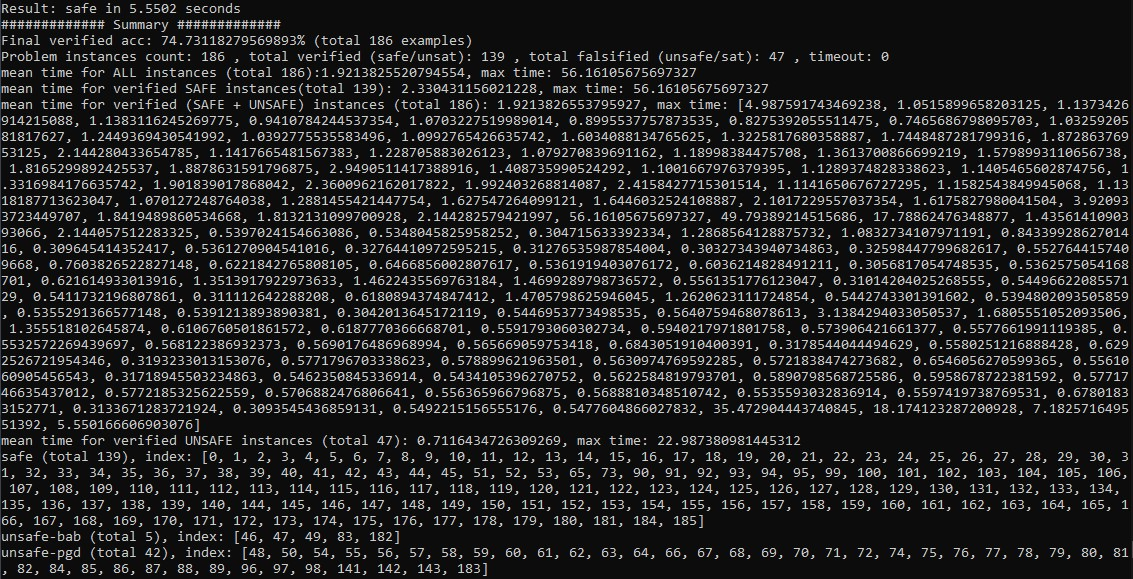
\includegraphics[scale=0.6]{alphabeta.jpg}
\newline
Here, "total verified" and "total falsified" are the number of instances in which the benchmark returned a correct and incorrect answer, respectively. We can also notice a timeout of 0, which means that none of the instances timed out during the verification process.

\subsection{Nnenum}
NNenum\cite{nnenum} is a high performance neural network verification tool. It uses multiple layers of abstractions in order to quickly verify neural networks without the cost of completeness. During VNN-COMP 2020, nnenum was the fastest running tool. Even though every contestant ran their tool on their own hardware, nnenum's speed is attributed to several algorithmic optimizations\cite{bak2021nfm}.
\newline
Prerequisites: 
\begin{itemize}
    \item Docker
    \item Python
\end{itemize}
To install nnenum, we first must clone the GitHub repository from the following address:  \url{https://github.com/stanleybak/nnenum}.
Next, we need to run the following command to build the tool using Docker:
\begin{verbatim}
    docker build . -t nnenum_image
\end{verbatim}
This will install all the prerequisites such as the required Python libraries.
\newline
Now that nnenum is installed, we can run it. First we need to run the following command:
\begin{verbatim}
    docker run -it nnenum_image bash
\end{verbatim}
This will start the shell in which nnenum is going to run.
\newline
In order to run onnx and vnnlib files one-by-one, we can use the follwing command from within this shell:
\begin{verbatim}
    python3 -m nnenum.nnenum examples/acasxu/data/ACASXU_run2a_3_3_batch_2000.onnx
    examples/acasxu/data/prop_9.vnnlib
\end{verbatim}
Alternatively, to run all the onnx and vnnlib files for ACAS Xu, we need to run the Python script located at examples/acasxu/acasxu\textunderscore all.py using the following command:
\begin{verbatim}
    python3 acasxu_all.py
\end{verbatim}
After running, nnenum saves the results in \verb|examples/acasxu/results/full_acasxu.dat|, which is a file that contains the verdict for every instance and looks like this:
\begin{verbatim}
1_1	1	holds	0.9043560099999013
1_2	1	holds	0.7880940459999692
1_3	1	holds	0.9245396309997886
5_9	1	holds	2.6333773339997606
1_1	2	holds	0.9800955360001353
1_2	2	violated	0.6960424779999812
1_3	2	violated	1.2031206550000206
1_4	2	violated	0.8025689860000966
1_5	2	violated	0.6941987039999731

...

5_7	4	holds	0.5372130199998537
5_8	4	holds	0.5712843749997774
5_9	4	holds	0.54370307399995
1_1	5	holds	1.5234227890000511
1_1	6	holds	5.243353473999832
1_9	7	violated	0.7887507830000686
2_9	8	violated	0.68229071199994
3_3	9	holds	3.115485338000326
4_5	10	holds	1.0181782939998811
\end{verbatim}
"Holds" means that the instance returned the correct answer and "violated" means that the instance returned the wrong answer.
\clearpage

\section{Experimental Results}
\begin{tabular}{c c c c c c c}
    \hline
    \# & Tool & Verified & Falsified & Penalty & Score & Percent \\
    \hline
    1 & nnenum & 139 & 47 & 0 & 1860 & 100\% \\
    2 & \alpha - \beta -CROWN & 139 & 47 & 0 & 1860 & 100\%
\end{tabular}
\newline \newline
Alpha-beta-CROWN ran for approximately 5-6 minutes before returning the final answer and nnenum ran for 4 minutes before returning the answer.\newline
From our analysis, both tools have managed to get a perfect score. The column "Verified" indicates how many instances the tool detected where the benchmark gave the correct answer. In the tool results, this is also referred to as "safe".
\newline 
The column "Falsified" indicates how many instances the tool detected where the benchmark gave the wrong answer. In the tool results, this is also referred to as "unsafe".
\newline
None of the tools received a penalty because they both correctly evaluate the answers given by the benchmark, without missing any deadlines. Thus, they both received a 100\% rating with a perfect score of 1860. The score is calculated as follows:\newline
\[Verified*10+Falsified*10-Penalty*150\]
These results match the official results from VNN-COMP23 \cite{vnn}.
The raw results from our testing can be found at the GitHub repository: \url{https://github.com/Vaduva-Vlad/ProiectVF}
\subsection{Obstacles encountered}
Although the process of running both tools is fairly smooth, we encountered a couple of problems along the way:
\begin{itemize}
    \item Alpha-beta-CROWN runs only on NVidia graphics cards. As such, the tool could only be run by the team members who have an NVidia graphics card.
    \item Alpha-beta-CROWN had a more complicated and error-prone installation process, requiring the installation of miniconda, Auto-LiRPA and the tool itself.
    \item Nnenum had to be run twice, because the first run returned an error on one of the instances. However, subsequent runs were successful, so we decided to give nnenum the maximum score.
    \item We've managed to install nnenum only on Windows, as the Docker installer did not work on Linux and manual installation returned many errors.
\end{itemize}
\section{Conclusions}
ACAS Xu is collision avoidance system that aims to increase the safety of air traffic. However, as suggested by our tests, the accuracy of the model (74.73\%) should be higher in order to reach this goal. This is why neural network verification is important. It is an important step towards assuring that the neural network is safe to use before integrating it into the aircraft. It is also a cost-saving measure as it reduces the failure rate in physical planes and lowers the number of materials wasted.
\newline
Measuring the accuracy of neural network verification tools is important, because it provides a continuous tool-benchmark improvement. In order for the neural network results to be correct, the benchmark verification needs to be accurate as well.
\clearpage
\bibliography{sample}
\bibliographystyle{ieeetr}

\end{document}